\section{Partial identification}

Sometimes we cannot say much about how the world words. If I tell
you that $\cos x=1$ you would be at a loss to tell me exactly what
$x$ is. You could say that $x=2\pi n$, for some integer $n$, but
not anything else. The situtation is bad, but could have been worse.
You do know something about $x$ after all; in the worst case scenario,
you would only know that $x\in\mathbb{R}$. You have \emph{partially
identifed} $x$. In contrast, if I tell you that $x\in[0,1]$, you
can immediatly answer that $x=0$, and you have \emph{identified}
$x$.

In general, iddentification is about answering questions on the form
``I know $K$ but want to know $W$, to what extent is this possible?''.
If this is possible for every $K$, there is a function $K\mapsto W$,
such as $f(K)=K^{2}$. Often tough, there are multiple possible $W$
compatible with $K$, and the mapping $K\mapsto\{W\}$ is set-valued,
such as $f(K)=\{\pm\sqrt{K}\}$.

Most identification problems in statistics and adjacent fields can
be analyzed using four spaces.
\begin{enumerate}
\item $\mathcal{F}$: A space of distributions. Think of these as latent
distributions underlying some phenomenon. 
\item $\mathcal{K}$: The space of what you know. This can be a multivariate
distribution, a set of marginal distributions, or perhaps some moments
of a distribution. Will demand that $K\in\mathcal{K}$ is the image
of an $F\in\mathcal{F}$ under some function. That is, there is a
surjective function $\mathcal{F}\to\mathcal{K}$. 
\item $\mathcal{\Theta}$: The parameter space of $\mathcal{F}$, a space
endowed with a surjective function $\Theta\to\mathcal{F}$. The parameter
space will sometimes contain information that cannot be deduced from
$\mathcal{F}$ itself, that is, the mapping $\theta\mapsto F$ does
not have to injective. 
\item $\mathcal{W}$: The space of what you want to know. The quantity we
wish to know is a function of $\theta$, henc there is a surjective
function $\mathcal{F}\to\mathcal{K}$. 
\end{enumerate}
The mappings above induce a set-valued map $H:\mathcal{K}\to\mathcal{W}$,
the\emph{ identification region} for $F$ \parencite{Manski2003-aq}.
Figure \ref{fig:partial identifiaction situation-1} shows the situtation
using a commutative diagram. 

\begin{figure}
\noindent \begin{centering}
\[
\begin{tikzcd}
\mathcal{F} \arrow[twoheadrightarrow]{r} & \mathcal{K} \arrow[dashed]{d}{H} \\
\Theta      \arrow[twoheadrightarrow]{u} \arrow[twoheadrightarrow]  & \mathcal{W}
\end{tikzcd}
\]
\par\end{centering}
\caption{\label{fig:partial identifiaction situation-1}The situation of partial
identification analysis. The double-headed arrows ($\twoheadrightarrow$)
denote surjections, the dashed arrow ($\protect\dashrightarrow$)
denotes the induced map.}
\end{figure}

Identification analysis is usually not presented in this formal way,
but is fruitful for three reason. First, it makes a clear a connection
between the seemingly disparate uses of the word ``identification''
across the stastical, medical, econonomic and sociological literutures.
Second, it allows us to state results using little notation and words.
For instance, $H(F)\subseteq A$ means that $A$ contains the identification
region of $F$. Third, it is possible to prove some general results
about these problems. 

As is customary in partial identification analysis, we ignore sampling
error \parencite{Manski2003-aq}. Making this assumption reduces the complexity
of the problem a lot. 

Identification analyses come in three forms, depending on which maps
are identities. 
\begin{description}
\item [{Convenience~identification}] When statisticians talk about identifiability
they usually think about convenience. Unidentified parameters make
estimation difficult and is a prerequisite for most asymptotic results.
In this case, the interpretation of the parameters are of no consequence.
In this case, both $\Theta\to\mathcal{W}$ and $\mathcal{F}\to\mathcal{K}$
are identity maps. We know $F$ and wish to know $\theta$. 
\item [{Space~of~distributions}] When $\Theta$ can be be identified
with the space of distributions $\mathcal{F}$, we are dealing with
partial identification of probability measures. In this setting, $F\in\mathcal{F}$
is the true, latent distribution, but we only observee some $K=\Psi(F)$.
We are usually not interested in getting to know $F$ itself, but
rather some sumary such as a correlation. A famous example is the
error-in-variables regression problem, considered below.
\item [{Structural~parameters}] Sometimes you want to say something about
parameters that are in extraprobabilistical, that is, they cannot
be encoded by probability measures. In problems of this type the spaces
$\Theta$ and $\mathcal{F}$ are distinct. The most famous example
is causal inference, where different causal assumptions can produce
identical joint distributons. 
\end{description}

\subsection{Convenience identification}

Identification is usually about parameterizations. A parameterization
is just a convenient way to represent an object, and we usually want
each representation to be unique. We want parameterizations since
probabilities is difficult beast to work with directly, but tuples
of reals are easy to handle. Let $\mathcal{P}$ be family of probability
measures and $\theta:\text{\ensuremath{\Theta\to\mathcal{P}}}$ a
surjective function on some parameter space $\Theta$. We will call
$\theta$ a parameter and say it is\emph{ identified }if $\theta$
is injective. 
\begin{example}
\label{exa:normal unidentified}Let $\Theta=[0,\infty)$ and map $\theta$
to the the probability distribution of a mean-zero normal variable
with standard deviation $\theta$. Then $\theta$ is injective, hence
identified. On the other hand, if $\Theta=\mathbb{R}$ and $\theta$
maps to the mean-zero normal probability with standard deviation $|\theta|$,
$\theta$ is not identified. For instance, both $-1,1$ maps to the
the standard normal probability.
\end{example}


\subsection{Partial identification of distributions}

In partial identification of probability distributions, the spaces
$\mathcal{F}$ and $\Theta$ of \ref{fig:partial identifiaction situation-1}
are equal. While partial identification is important in several fields,
econometricians have been more active than others in studying it.
Two important books are those of \cite{Manski1999-ab,Manski2003-aq},
and \cite{Tamer2010-rj} is a more recent review. The motivation
for partial identification analyses is a principle connecting assumptions
with believeability \cite[p. 1]{Manski2003-aq}:
\begin{quote}
\emph{The Law of Decreasing Credibility: }The credibility of inference
decreases with the strength of the assumptions maintained.
\end{quote}
There is a trade-off between credibility and assumptions. Not only
can strong assumptions provide identifiability, but models that are
much easier to deal with computationally and mathematically. It is
easier to compute a linear regression with normal erros than one with
\emph{t}-distributed errors, and confidence intervals are exact only
in the former case. Moreover, adding assumptions can make models much
easier to interpret; the linear regression model $Y=\alpha+\beta X+\epsilon$
is as clear as day, $Y=\alpha+\beta X+\delta e^{\sin X}\Gamma(X)\epsilon$
is obscure. 
\begin{example}[Error-in-variables regression model]
 Let $Y,Z$ be two variables of finite variance, $Y$ observable
and $Z$ latent. We want to know $\beta=\Cov(Y,Z)/\Var(Z)$, that
is, the regression coefficient of $Z$. Let $X=Z+\eta$ an observed
variable, where $\eta$ has finite variable and is uncorrelated with
$X$ and $Z$. We know know the the second moments moments $\Var X$
and $\Cov(Y,X)$, i.e., $K=(\Var X,\Cov(Y,X)$. What can we say about
$\beta$? 

Define $\beta^{\star}=\Cov(X,Y)/\Var X$. Since $\Var X=\Var Z+\Var\eta$
and $\Cov(X,Y)=\Cov(Z+\eta,Y)=\Cov(Z,Y),$we find
\[
\beta^{\star}=\frac{\Cov(Z,Y)}{\Var Z+\Var\eta}=\frac{\beta}{1+\frac{\Var\eta}{\Var Z}}=\frac{\Var Z}{\Var X}\beta.
\]
If we make the assumption that $m\leq\Var Z\leq\Var X$, we obtain
the identification region $H=\beta^{\star}[1,\Var X/m)$. 
\end{example}


\subsubsection{When you know some correlations}

Let $X,Y,Z$ be random variable with unit variance. Assume you know
$\rho_{12}=\Cov(X,Y)$, $\rho_{23}=\Cov(Y,Z)$. What can you say about
$\rho_{13}=\Cov(X,Z)$? This problem is known from the literature
on matching \parencite{Rassler2012-rp}.You need to fill out
\[
\Phi=\left[\begin{array}{ccc}
1 & \rho_{12} & ?\\
\rho_{12} & 1 & \rho_{23}\\
\text{\ensuremath{?}} & \rho_{23} & 1
\end{array}\right]
\]
subject only to the constaint that $\Phi$ is positive definite. 
\begin{proposition}
\label{prop:correlation identification}The following identification
sets are true.
\begin{enumerate}
\item When $\rho_{23}$ and $\rho_{12}$ are known, the identification region
for $\rho_{13}$ is the open interval
\begin{equation}
\rho_{13}\in\rho_{12}\rho_{23}\pm\sqrt{\rho_{12}^{2}\rho_{23}^{2}-\rho_{23}^{2}-\rho_{12}^{2}+1}.\label{eq:identification set correlation}
\end{equation}
In particular, when $\rho_{12}=\rho_{23}=\rho$, the partial identification
set is $(2\rho^{2}-1,1)$. 
\item If only $\rho_{12}$ is known, the identification region for $(\rho_{13},\rho_{23})$
is the ellipse width $2\sqrt{1+\rho_{12}}$ and height $2\sqrt{1-\rho_{12}}$,
rotated $\pi/4$ degrees. In particular, when $\rho_{12}=0$, the
identification set is the open Euclidean unit ball in $\mathbb{R}^{2}$.
\end{enumerate}
\end{proposition}

\begin{proof}
We will use Sylvester's criterion \parencite{Gilbert1991-ch}. Applied
to a $3\times3$-matrix $A$, it says that $A$ is positive definite
if and only if (i) $A_{11}$ is positive, (ii) the determinant of
the $2\times2$ upper-left corner of $A$ is positive, and (iii) the
determinant of $A$ itself is positive. 

Since $\Phi_{11}=1$, (i) satisfied, and so is (ii) since $\rho_{12}$
is a correlation. The determinant of $\Phi$ is
\begin{eqnarray*}
\det\Phi & = & (1-\rho_{23}^{2})-\rho_{12}(\rho_{12}-\rho_{23}\rho_{13})+\rho_{13}(\rho_{12}\rho_{23}-\rho_{13}).
\end{eqnarray*}
Fixing $\rho_{12}$ and $\rho_{23}$, this is positive and if the
quadratic functin $\rho_{13}^{2}-2(\rho_{12}\rho_{23})\rho_{13}+(\rho_{23}^{2}+\rho_{12}^{2})<0$.
Since this equation has roots $\rho_{12}\rho_{23}\pm\sqrt{\rho_{12}^{2}\rho_{23}^{2}-\rho_{23}^{2}-\rho_{12}^{2}+1}$,
equation (\ref{eq:identification set correlation}) follows. As for
$\rho_{12}=\rho_{23}=\rho$, the limits are $\rho^{2}\pm\sqrt{(\rho^{2}-1)^{2}}$,
or, equivalently, $(2\rho^{2}-1,1).$

Time to take on (ii). Fix $\rho_{12}=\rho$ and define $x=\rho_{13},y=\rho_{23}$.
Then equation (\ref{eq:identification set correlation}) can be rearranged
to
\begin{equation}
y=x\rho+\sqrt{1-\rho^{2}}\sqrt{1-x^{2}}.\label{eq:ellipse eq1}
\end{equation}
Subtracting $x\rho$ on both sides and squaring yields $(y-x\rho)^{2}=(1-\rho^{2})(1-x^{2}).$
In expanded form, this is $y^{2}-2xy\rho+x^{2}\rho^{2}=1-\rho^{2}-x^{2}+x^{2}\rho^{2}$,
which can be rearranged to $y^{2}-2xy\rho+x^{2}=1-\rho^{2}$. 

The formula for an ellipse with width $2a$ and height $2b$, rotated
$\theta$ degrees is

\[
\frac{(x\cos\theta+y\sin\theta)^{2}}{a^{2}}+\frac{(x\sin\theta-y\cos\theta)^{2}}{b^{2}}=1.
\]
When $\theta=\pi/4$, $\cos\theta=\sin\theta=1/\sqrt{2}$, hence 
\begin{equation}
\frac{(x+y)^{2}}{2a^{2}}+\frac{(x-y)^{2}}{2b^{2}}=1\label{eq:pi/4-rotated ellipse}
\end{equation}
is the ellipse with width $2a$ and height $2b$ rotated $\theta=\pi/4$
degrees.

Take $a=\sqrt{1+\rho_{12}}$ and $b=\sqrt{1-\rho_{12}}$ and plug
them into (\ref{eq:pi/4-rotated ellipse}) to verify it is equivalent
to $y^{2}-2xy\rho+x^{2}=1-\rho^{2}$. Since each $x,y$ in the ellipse
will satisfy the limits of (\ref{eq:identification set correlation}),
we are done.
\end{proof}
\begin{figure}
\noindent \begin{centering}
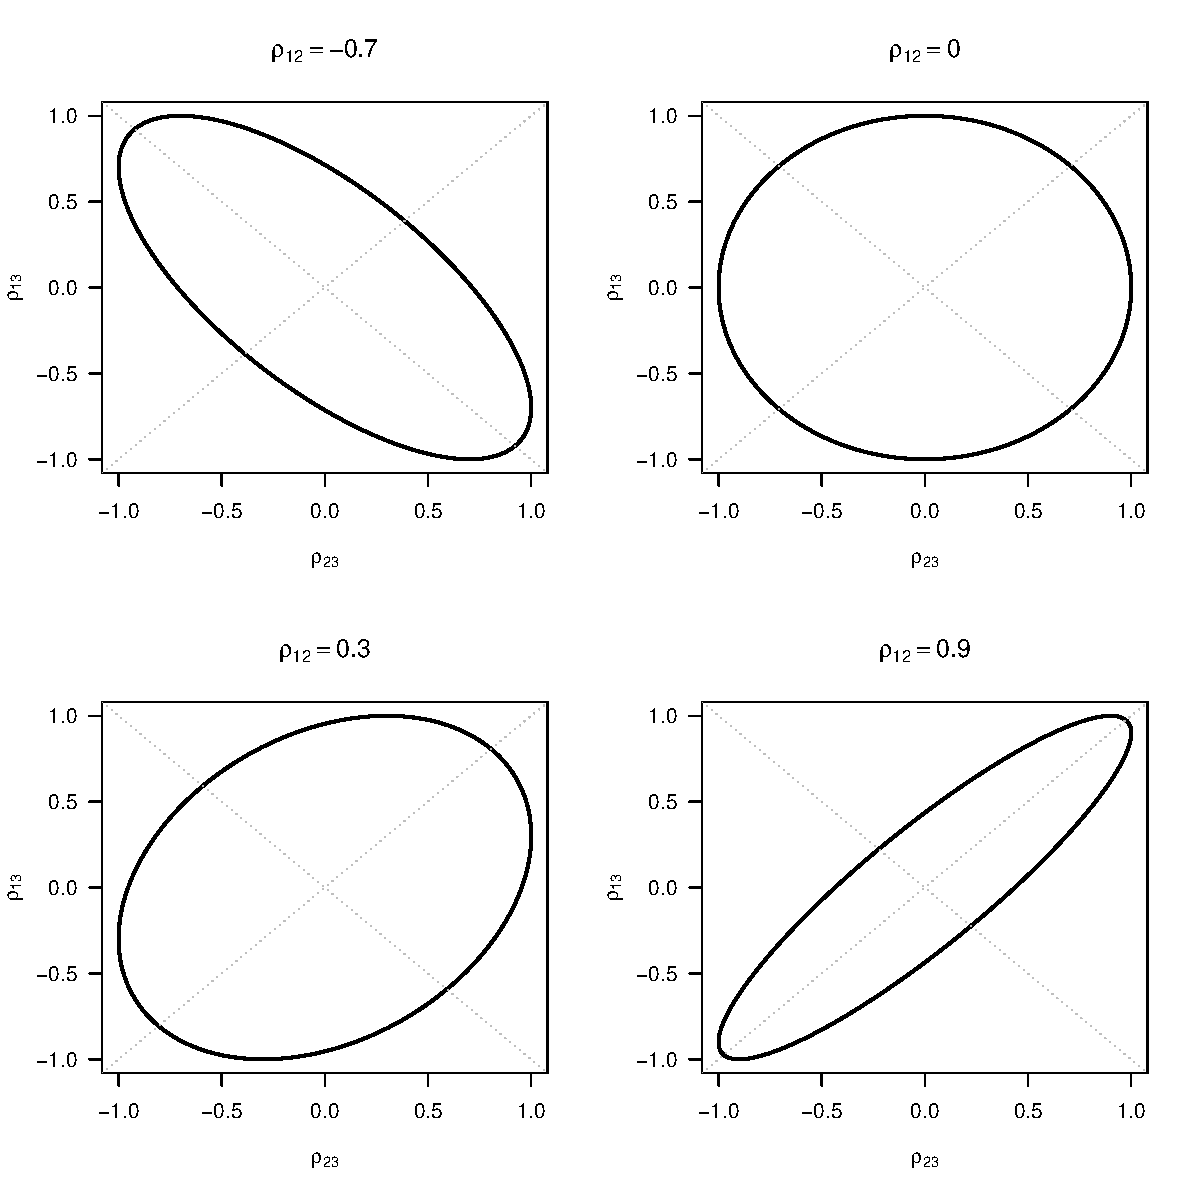
\includegraphics[scale=0.4]{chunks/rho}
\par\end{centering}
\caption{The ellipses of Proposition (\ref{prop:correlation identification})
for a selection of correlations $\rho_{12}$.}
\end{figure}
%
\begin{example}[{\cite[p. 10]{Rassler2012-rp}}]
 Assume 
\[
\Phi=\left[\begin{array}{ccc}
1 & 0.9 & \rho_{13}\\
0.9 & 1 & 0.8\\
\rho_{13} & 0.8 & 1
\end{array}\right]
\]
Applying Propositon \ref{prop:correlation identification} gives us
the identification set $(0.4585,0.9815)$. We do know something about
the correlation after all.
\end{example}


\subsubsection{How many people know basic scientific facts?}
\begin{quote}
\textbf{\emph{Question 3}}: Does the Earth go around the Sun, or does
the Sun go around the Earth?

\medskip

$\bigcirc$ Earth goes around the Sun.

$\bigcirc$ Sun goes around the Earth.
\end{quote}
The National Science Board \citeyear[Table 7-8]{National_Science_Board2014-yl}
reports that a shockingly high percentage of people answer this question
incorrectly. Only $74$\% of American adults answered correctly, while
an even worse $66$\% of European Union residents answered correctly.
South Koreans did slightly better, at $86$\%. But the truth percentage
of Americans who know the Earth goes around the Sun is probably even
lower than $74$\%. A non-human monkey would select either option
with equal probability, and some humans probably do this too. The
base-line of no knowledge is $50$\% correct answers. So what's the
real percentage of people of who knows that the Earth goes aroun the
Sun? 

A popular way to model people's state of knowledge is to use probability
distributions. Imagine everyone has a probability distribution over
the answers to Question 3. Denote this distribution $c$ and the proposition
that the Earth goes around the Sun by $A$. Then the knowledge of
a person is captured by $c(A)$. 

We want to know the percentage of people that knows the answer to
$A$. Even if we knew everyone's probability distributions $c$, the
answer to this question is not completely straightforward. Knowing
or not knowing must involve a cutoff. For instance, you could claim
that you know $A$ when you are at least $95\%$ certain of $A$ and
$A$ is true. This cutoff is arbitrary, and could equally well have
been $75\%$, $99\%$, or anything else. A natural restriction is
to deman a certainty of more than $50\%$, but otherwise any percentage
appears defensible. To take this arbitrariness of the cutoffs into
account, let us say that a person $\alpha$-knows $A$ if $c(A)>\alpha$
and $A$ is true. Now we can restate goal: We want to find the percentage
of the population that $\alpha$-knows that the Earth orbits the sun.

To model all of this, let $c$ be a credence function sampled according
to $Q$ and $X\mid c$ sampled according to $c$,

\[
c\sim Q,\quad X\mid c\sim c.
\]

The next step is to decide on the possible space of distributions
$Q$. \cite[Chapter 2, endnote 28]{Caplan2018-oj} assumes that every
person either knows $A$ with certainty or guesses with $50/50$ odds.
In this case, $Q$ can be a parameterized by $\gamma$, the proportion
who knows for certain. Then $1-\gamma=2(1-P(A))$, hence $\gamma=1-2(1-P(A))=2P(A)-1$.
When $P(A)=0.74$ we get $\gamma=0.48$, hence just below $50\%$
of the population $\alpha$-knows the Earth goes aroun the Sun when
$\alpha\geq0.5$.

In the spirit of \cite{Manski2003-aq}, we will make no assumption
about $Q$. Define the parameter $\Psi_{\alpha}(Q)=Q(c(\textrm{correct answer})>\alpha).$ 
\begin{proposition}
\label{prop:guessing regions}Let $P(X=1)=\beta\in(0,1)$. Then 
\[
H_{\alpha}(\beta)=\begin{cases}
[(\beta-\alpha)/(1-\alpha),1], & \textrm{when }\beta>\alpha,\\
(0,1), & \textrm{when }\beta=\alpha,\\{}
[0,\beta/\alpha], & \textrm{when }\beta<\alpha.
\end{cases}
\]
\end{proposition}

\begin{proof}
Assume $\beta>\alpha$. Let $A$ be the event that $c(1)\leq\alpha$
and $B$ the event that $c(1)>\alpha$. Denote $P(X=1\mid A)=\alpha-\epsilon$,
where $\epsilon\in[0,\alpha]$, assume $P(X=1\mid B)=\beta+\delta$,
$\delta\in[0,1-\beta]$, and denote $P(B)=q$. By the law of total
probability,
\[
P(X=1)=P(B)(\beta+\delta)+P(A)(\alpha-\epsilon).
\]
Since $\beta=P(X=1)$, $P(B)=q$, and $P(A)=1-q$, we get $\beta=q(\beta+\delta)+(1-q)(\alpha-\epsilon).$
Rearrange to get $q=(\beta-\alpha+\epsilon)/(\beta-\alpha+\epsilon+\delta)$.
This is maximized when $\delta=0$, when $q=1$. It is minimized when
$\epsilon=0$ and $\delta=1-\beta$, when $q=(\beta-\alpha)/(1-\alpha).$

That $E(\alpha)=(0,\beta/\alpha]$ when $\alpha\geq\beta$ can be
verified by duality. For now $1-\alpha\leq1-\beta$, and we can use
the same analysis as above when regarding $2$ as the right answer.
Hence the maximum is $1$ and the minimum is $(1-\beta-(1-\alpha))/(1-(1-\alpha)=(\alpha-\beta)/\alpha$.
Turn back to the case when $1$ is the right by forming $1-(0,(\alpha-\beta)/\alpha)=(0,\beta/\alpha].$
\end{proof}
\begin{figure}
\noindent \begin{centering}
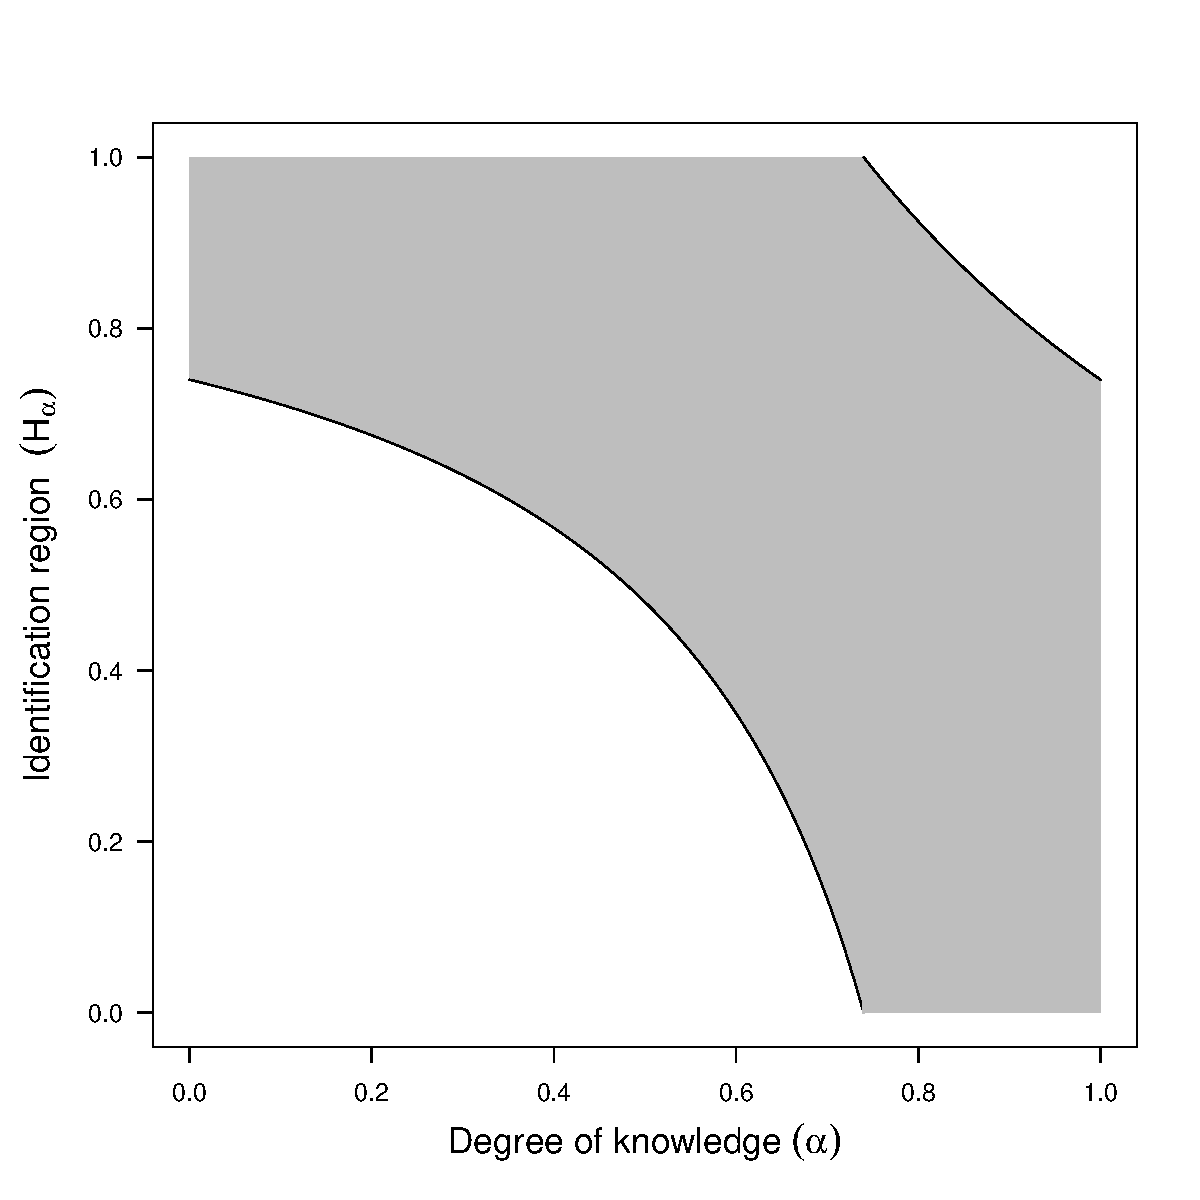
\includegraphics[scale=0.5]{chunks/knowing}
\par\end{centering}
\caption{\label{fig:Identification-regions-guessing}Identification regions
when $P(A)=0.74$.}
\end{figure}

The identification regions of Proposition \ref{prop:guessing regions}
are wide. Figure \ref{fig:Identification-regions-guessing} tells
the story when $P(A)=0.74$. In particular, when $\alpha=0.95$, we
get $E(\alpha)=[0,0.78]$, meaning anything between $0\%$ and $78\%$
of the population knows $A$ with mimimum $95\%$ certainty. If we
choose the low $\alpha=0.6$, we get $E(\alpha)=[0.35,1]$, so at
least $35\%$ of the population knows $A$ with minimum $60\%$ percent
certainty. 

\subsection{Identification of structural parameters}

Structural parameters are extra-probabilistical; they encode something
about the world the isn't captured in any probability distributions.
Causal inference is about structural parameters. The joint distribution
of $(X,Y)$ does not tell us if $X$ causes $Y$. The causal information
is encoded in e.g. a causal graph \parencite{Pearl2009-zf} or a system
of counterfactuals \parencite[Chapter 4]{Pearl2016-tc}. A related example
is identifacation of structural parameters is from psychometrics.
In geneal, several structural equation models can give rise to exactly
the same joint distribution, but with highly disparate interpretations
\parencite{Raykov2001-ap}. Econometrics have perhaps the most famous
identification problem, sometimes called the identification problem
in econometrics \parencite{Manski1999-ab}.
\begin{example}[The identification problem in econometrics]
 Let $p$ be the price and $q$ the quantity of some good. Assume
the linear supply and demand functions
\begin{eqnarray*}
s(p) & = & \alpha_{s}+\beta_{s}p+\epsilon_{s}\quad\textrm{(supply)},\\
d(p) & = & \alpha_{d}+\beta_{d}p+\epsilon_{d}\quad\textrm{(demand).}
\end{eqnarray*}
Here $s(p)$ is the quantity supplied at the price $p$, $d(p)$ is
the quantity demanded at the price $p$, and $\epsilon_{1},\epsilon_{2}$
are uncorrelated error terms with zero mean and variances $\sigma_{1}^{2},\sigma_{2}^{2}$.
If prices are in equilibrium, $q=s(p)=d(p)$, where $q$ is the quantity
of the good, hence
\[
q=\alpha_{s}+\beta_{s}p+\epsilon_{1}=\alpha_{d}+\beta_{d}p+\epsilon_{2}.
\]
We want to know the supply and demand functions, or equivalently,
$(\alpha_{s},\beta_{s},\alpha_{d},\beta_{d})$. We know the mean $\mu$
and covariance $\Sigma$ of $(p,q)$:
\end{example}

\begin{eqnarray*}
\mu & = & \left(\frac{\alpha_{d}-\alpha_{s}}{\beta_{s}-\beta_{d}},\frac{\beta_{s}\alpha_{d}-\beta_{d}\alpha_{s}}{\beta_{s}-\beta_{d}}\right)\\
\Sigma & = & \frac{1}{(\beta_{s}-\beta_{d})^{2}}\left[\begin{array}{cc}
\sigma_{1}^{2}+\sigma_{2}^{2} & \beta_{d}\sigma_{1}^{2}+\beta_{s}\sigma_{2}^{2}\\
\beta_{s}\sigma_{1}^{2}+\beta_{s}\sigma_{2}^{2} & \beta_{d}^{2}\sigma_{1}^{2}+\beta_{s}^{2}\sigma_{2}^{2}
\end{array}\right]
\end{eqnarray*}
Here we have $5$ knowns $(\mu_{1},\mu_{2},\Sigma_{11},\Sigma_{22},\Sigma_{12})$
and $6$ unknowns, $x=(\alpha_{s},\beta_{s},\alpha_{d},\beta_{d},\sigma_{1}^{2},\sigma_{2}^{2})$
in a system of quadratic equations. This system of equations has no
unique solution, and several identifying restrictions have been proposed.
See \cite[Chapter 6]{Manski1999-ab} for details.